\documentclass{article}
\usepackage{graphicx}
\usepackage{amsmath, amssymb}
\usepackage{mathtools}
\usepackage{derivative}
\usepackage{enumitem}
\usepackage{amsfonts}

\newcommand{\R}{\mathbb{R}}
\newcommand{\C}{\mathbb{C}}
\newcommand{\M}{\mathcal{M}}
\newcommand{\F}{\mathcal{F}}
\newcommand{\ex}{\textit}
\newcommand{\sol}{\\ \textbf{Solution: }}
\newcommand{\proof}{\\ \textbf{Proof: }}
\newcommand*{\eqdef}{\ensuremath{\overset{\mathclap{\text{\tiny def}}}{=}}}
\usepackage{graphicx} % Required for inserting images
\newcommand{\ssubset}{\subset\joinrel\subset}
\newcommand{\ppdv}[2]{\frac{\partial^2 #1}{\partial{#2}^2}}

\title{Exercises \- Mathematical quantum theory}
\author{Simone Coli \- 6771371}
\date{Sheet 7}
\begin{document}
\maketitle

\section{Exercise}
Let $ V: \R^3 \to \R$ be a potential satisfying $V \in L^p(\R^3)$ for some $2<p\leq \infty$. Let us now consider the Schrödinger operator
\[
    H = -\Delta + V, \quad D(H) = H^2 (\R^3)
\]
on $\mathcal{H} = L^2(\R^3)$. We want to show that $H: D(H) \to L^2 (\R^3)$ is well-defined and symmetric.

With well-defined we mean that if $\psi \in H^2(\R^3)$ then $H\psi \in L^2(\R^3)$, which in this contest means that $\Delta \psi \in L^2(\R^3)$ and $V \psi \in L^2(\R^3)$. The first follow from the definition of $H^2(\R^3)$ spaces. We are left to prove that 
\[
    \int_{\R^3} |V \psi|^2 dx \leq \infty.
\]
Let us consider the two sets in which $|V|$ is bigger and smaller than $1$: $\Omega^> := \{ x \in \R^3 | |V(x)| > 1 \}$ and $\Omega^< := \{ x \in \R^3 | 0< |V(x)| < 1 \}$
\[
    \begin{split}
        \int_{\R^3} |V|^2 |\psi|^2 dx &= \int_{\Omega^>} |V|^2 |\psi|^2 dx + \int_{\Omega^<} |V|^2 |\psi|^2 dx \leq\\
        & \leq \int_{\Omega^>} |V|^p |\psi|^2 dx + \int_{\Omega^<} |\psi|^2 dx
    \end{split}
\]
since in one case multiplying $V$ by himself makes it smaller than it was before bounded from above by $1$, while in the other it makes it bigger than before. From here we already have that the term on $\Omega^<$ is already in $L^2(\R^3)$ by definition we now need to work on the other one.\\
Using Hölder's inequality we have that
\[
    \begin{split}
        \int_{\Omega^>} |V|^2 |\psi|^2 dx & \leq  \| |V|^p \|_1 \cdot \| \psi^2 \|_\infty = \\
        & = \int_{\Omega^>} |V|^p dx \cdot \mbox{ ess} \sup_{\Omega^>}{|\psi|^2}
    \end{split}
\]
We know that $V \in L^p(\R^3)$ then it is bounded. Now what is left is to check that the essential supremum of $\psi$ is bounded, which it is from Sobolov embedding theorem. From this we know that $\psi \in C^0_\infty(\R^3)$ and therefore that $|\psi|^2 \in C^0_\infty (\R^3)$. Because of that we know that the function is bounded and therefore is in $L^\infty (\R^3)$.

Let us now show that the operator is symmetric when $\psi \in H^2(\R^3)$:
\[
    \begin{split}
        \langle \psi, H \psi \rangle &=  \langle \psi, (-\Delta + V) \psi \rangle = \langle \psi, - \Delta \psi \rangle + \langle \psi, V \psi \rangle = \\
        &= \langle \hat \psi,  -k^2 \hat\psi \rangle + \int_{\R^3} \overline{\psi} V \psi dx = \int_{\R^3} \overline{-k^2 \hat \psi} \hat \psi dx + \int_{\R^3} \overline{V \psi} \psi dx =\\
        &= \langle -k^2 \hat \psi, \hat \psi \rangle + \langle V \psi,  \psi \rangle = \langle -\Delta \psi, \psi \rangle + \langle V \psi, \psi \rangle
    \end{split}
\]
since both $V$ and $k$ are real valued. Which proves the claim.

\section{Exercise}
Let $d\geq 3$ with $V = v + w$ such that $v \in L^{d / 2} (\R^d)$ and $w \in L^\infty(\R^d)$, given the quadratic from
\[
    q(\psi) = \langle \nabla \psi, \nabla \psi \rangle + \langle \psi, V \psi \rangle
\]
defined on $Q= H^1 (\R^d)$.

a) We want to show that $q$ is actually bounded from below. Let us start with
\[
    q(\psi) = \| \nabla \psi \|_2 + \int_{\R^d} |\psi|^2 v + \int_{\R^d} |\psi|^2 w dx
\]
From the definition of $L^\infty (\R^d)$ we have that $w \in (-\| w \|_\infty, \| w\|_\infty)$ meaning it can be bounded from below by $-\| w \|_\infty$. Moreover, $\| \nabla \psi \|_2>0$ by definition of norm. It is left to shoe that the last term is bounded from below. 
To do that, let us consider two subspaces of $\R^d$: $\Omega^+ = \{ x \in \R^d | v(x)\geq 0 \}$ and $\Omega^- = \{ x \in \R^d | v(x)<0 \}$ then 
\[
    \begin{split}
        \int_{\R^d} |\psi|^2 v dx &= \int_{\Omega^+} |\psi|^2 v dx + \int_{\Omega^-} |\psi|^2 v dx = \int_{\Omega^+} |\psi|^2 v dx - \int_{\Omega^-} |\psi|^2 |v| dx
    \end{split}
\]
The first term is bounded from below by $0$. To show that also the second is bounded from below we use Hölder's inequality.
\[
    \| |\psi|^2 |v| \|_1  \leq \| |\psi|^2 \|_p \cdot \| v \|_q
\]
Let us choose $q = \frac{d}{2}$, then $p = \frac{d}{d-2}$, then
\[
    \| |\psi|^2 \|_p = {\left(\int_{\R^d} |\psi|^{\frac{2d}{d-2}}\right)}^{\frac{d}{d-2}} = {\| \psi \|}^2_{\frac{2d}{d-2}}  \leq C \| \nabla \psi  \|_2
\]
while by definition $v \in L^{d / 2}(\R^d)$ meaning that there exists $\bar x$ such that for some constant $M >0$, $M > v(\bar x)$. Meaning that
\[
    - \| |\psi|^2 |v| \|_1 =  - \int_{\Omega^-} |\psi|^2 |v| dx \geq - M C \| \nabla \psi  \|_2
\]
since $\psi \in H^1(\R^d)$, $\nabla \psi \in L^2(\R^d)$. From which it follows that $q(\psi)$ is bounded from below.
\section{Exercise}
Let $f : \R^d \to \C$ be a continuous function. On $\mathcal{H} = L^2(\R^d)$ we define the multiplication operator $( \M_f, D(\M_f) )$ on the domain
\[
    D(\M_f) = \{ \psi \in L^2(\R^d) : f\psi \in L^2(\R^d) \}
\]

a) We want to prove that $\sigma(\M_f) = \mbox{ran }f$ where $\mbox{ran }f$ is the range of $f$. To do so we look at the spectrum of the operator $\M_f - z = \M_{\frac{1}{f-z}}$. The domain of this operator will be defined as 
\[
    D(\M_{\frac{1}{f-z}}) := \{ \psi \in L^2 (\R^d) | \frac{1}{f-z} \psi \in L^2(\R^d) \} 
\]
this means that \\
\[
    \int_{\R^d} \frac{1}{|f-z|^2} |\psi(x)|^2 dx < \infty
\]\\
and this is true when $z \neq f(x)$. The resolvent will be
\[
    \rho(\M_f) = \{ z\in \C | z \neq f(x) \}
\]
while the spectrum is:
\[
    \sigma(\M_f) = \mbox{ran }f
\]

b) We want to find a function which is not constant by has point spectrum $\sigma_P = \{ a \}$ with $a \in \C$. A function with this property is just a function of the type:
\[
    f(x) = \begin{cases}
        a & x<0\\
        x + a & x \geq 0 
    \end{cases}
\]
\begin{figure}[!ht]
    \centering
    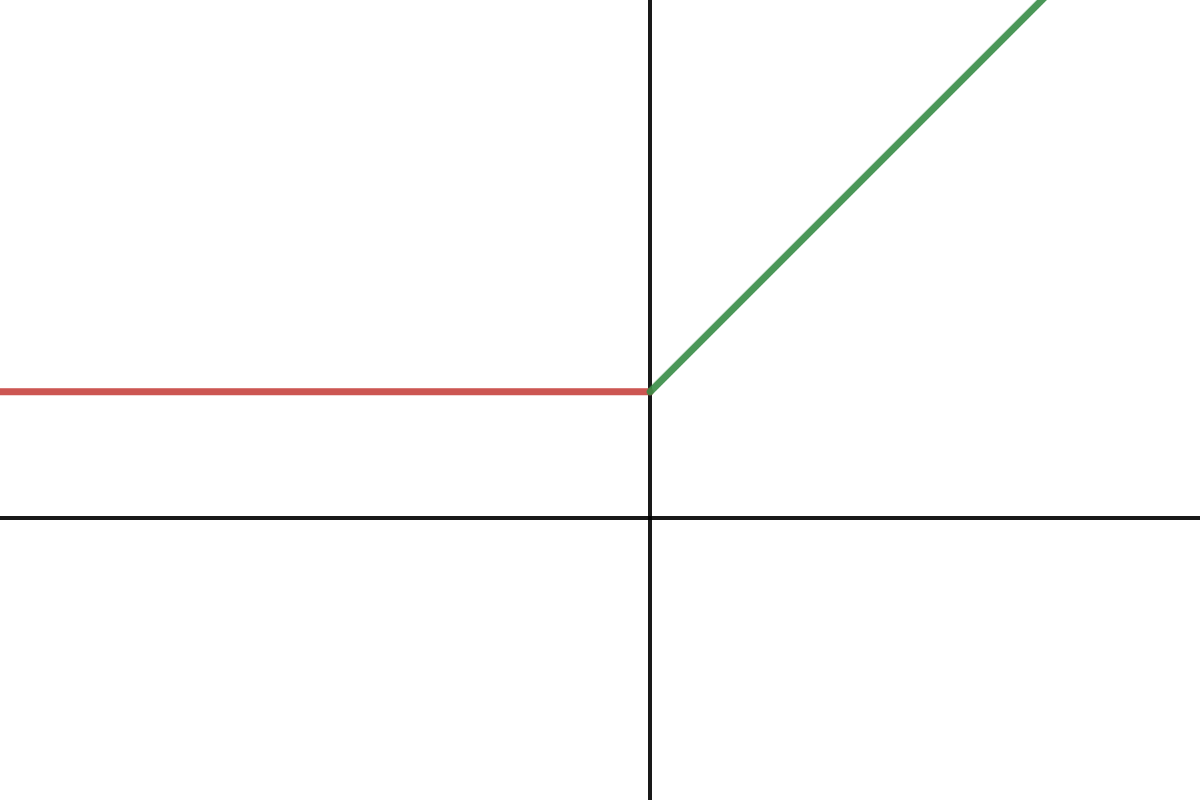
\includegraphics[width = 0.5 \textwidth]{TeX/IMG/desmos-graph.png}
\end{figure}\\
so that it has both continuous and point spectrum. In particular from what we found in part (a), we have $\sigma (\M_f) = \mbox{ran }f = \{ a\leq x \leq \infty \}$, where $\sigma_P(\M_f) = \{ a \}$ and $\sigma_C (\M_f) = {a < x \leq \infty}$.
\section{Exercise}
a) Let $U : \to \mathcal{H} \to \mathcal H $ be unitary and $(T, D(T))$ an unbounded operator. We want to show that 
\[
    \sigma(T) = \sigma(UTU^*), \quad \sigma_\#(T) = \sigma_\# (UTU^*)
\]
for any $\# \in \{ p,c,r \}$

From the previous exercise sheet we have that 
\[
    {(UTU* - z)}^{-1} = {(U(T-z)U^*)}^{-1} = U{(T-z)}^{-1} U^* \quad (*)
\]
if, and only if, $(T-z)$ is bijective. This means that if we consider the resolvent of $T$
\[
    \rho(T) = \{ z \in \C | T-z : D(T) \to \C \text{ is bijective with bounded inverse} \}
\]
\[
    \begin{split}
        \rho(UTU^*) &= \{ z \in \C | U(T-z)U^*  : D(UTU^*) \to \C 
        \text{ is bijective} \\
        & \text{with bounded inverse} \}\\
        &= \{ z \in \C | UTU^* -z  : D(T) \to \C \text{ is bijective with bounded inverse} \}
    \end{split}
\]\\
since $U$ is unitary and does not affect the $L^2(\R^d)$ norm. Then 
\[
    \sigma(T) = \C \setminus \rho(T)  = \C \setminus \rho({UTU^*}) = \sigma(UTU^*) 
\]\\
Moreover, from $(*)$ we have that the inverse of $UTU^* -z$ is the composition fo continuous functions by hypothesis, meaning that the inverse of such and operator must be bounded, since continuity implies boundness. Now since
\[
    \sigma (T) = \sigma_P(T) \sqcup  \sigma_C (T) \sqcup \sigma_R(T) = \sigma (UTU^*)
\]
the also $\sigma_{\#} (T) = \sigma_\# (UTU^*)$ since
\[
    \sigma (UTU^*)= \sigma_P(UTU^*) \sqcup  \sigma_C (UTU^+) \sqcup \sigma_R(UTU^*)
\]
is a disjoint union.

b) Let us consider the momentum operator $(-i d / dx, H^1(\R^d))$ on $L^2(\R^d)$. We want to find a unitary transformation which makes it a multiplication operator and the Fourier transform does exactly that. It transforms the momentum operator into the position operator, which is a multiplication operator.

c) Identify the spectrum, the point spectrum, and the continuous spectrum of
the momentum operator. From what we have seen in class, we know that the position operator has spectrum $\sigma(\M_x) = \R$ from part (a) of thi exercise we have that
\[
    \sigma(\M_x) = \sigma(\F \M_x \F^{-1}) = \R
\]
which follows from the fact that the Fourier operator is unitary and the fact that $M_p = \F \M_x \F^{-1}$. Meaning that it also as a pure continuous spectrum and an empty point spectrum. 
\end{document}